\documentclass[usenames,dvipsnames,tikz]{standalone}
\usepackage{amsmath,amssymb}
\usepackage{xcolor}
\colorlet{tBlue}{RoyalBlue!35!Cerulean}
\colorlet{tRed}{Red}
\usepackage{tikz}
\usepackage{standalone}
\begin{document}
	
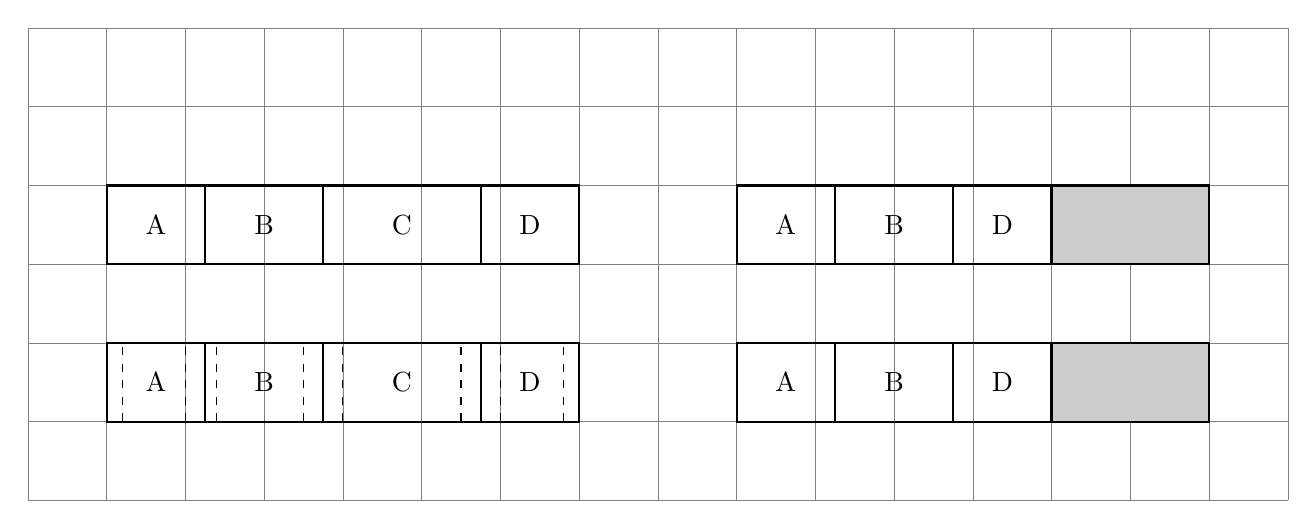
\begin{tikzpicture}
\draw [help lines] (-1,-1) grid (15,5);
% 1=0.1, 2=0.15, 3=0.2, 4=0.25, 5=0.3
% 6, 5, 4, 4, 3, 3, 2, 1, 1, 1.

\draw [thick] (0,0) rectangle (6,1);
\draw [thick] (0,2) rectangle (6,3);


% Bottom row - SCPP
\draw [thick] (1.25,0) -- (1.25,1);
\draw [thick] (2.75,0) -- (2.75,1);
\draw [thick] (4.75,0) -- (4.75,1);
\node at (0.625, 0.5) {A};
\node at (2, 0.5) {B};
\node at (3.75, 0.5) {C};
\node at (5.375, 0.5) {D};
\draw [dashed] (0.2,0) -- (0.2,1);
\draw [dashed] (1,0) -- (1,1);
\draw [dashed] (1.4,0) -- (1.4,1);
\draw [dashed] (2.5,0) -- (2.5,1);
\draw [dashed] (3,0) -- (3,1);
\draw [dashed] (4.5,0) -- (4.5,1);
\draw [dashed] (5,0) -- (5,1);
\draw [dashed] (5.8,0) -- (5.8,1);


% Top row - BPP
\draw [thick] (1.25,2) -- (1.25,3);
\draw [thick] (2.75,2) -- (2.75,3);
\draw [thick] (4.75,2) -- (4.75,3);
\node at (0.625, 2.5) {A};
\node at (2, 2.5) {B};
\node at (3.75, 2.5) {C};
\node at (5.375, 2.5) {D};



%---------------------------------------------------------------------

\draw [thick] (8,0) rectangle (14,1);
\draw [thick] (8,2) rectangle (14,3);


% Bottom row - SCPP
\draw [thick] (9.25,0) -- (9.25,1);
\draw [thick] (10.75,0) -- (10.75,1);
\draw [thick] (12,0) -- (12,1);
\filldraw[fill=black!20!white, draw=black, thick] (12,0) rectangle (14,1);
\node at (8.625, 0.5) {A};
\node at (10, 0.5) {B};
\node at (11.375, 0.5) {D};


% Top row - BPP
\draw [thick] (9.25,2) -- (9.25,3);
\draw [thick] (10.75,2) -- (10.75,3);
\draw [thick] (12,2) -- (12,3);
\filldraw[fill=black!20!white, draw=black, thick] (12,2) rectangle (14,3);
\node at (8.625, 2.5) {A};
\node at (10, 2.5) {B};
\node at (11.375, 2.5) {D};








\end{tikzpicture}

\end{document}